\documentclass[UTF8,fontset=mac]{ctexart}
\usepackage{fontspec}
\setCJKmainfont{PingFang SC}
\setCJKsansfont{PingFang SC}
\setCJKmonofont{PingFang SC}
\usepackage{amsmath,amssymb,amsthm}
\usepackage{graphicx}
\usepackage{hyperref}
\usepackage{geometry}
\geometry{margin=1in}
\usepackage{booktabs}
\usepackage{longtable}
\usepackage[numbers]{natbib}
\newtheorem{theorem}{定理}[section]
\newtheorem{definition}{定义}[section]
\newtheorem{proposition}{命题}[section]
\newtheorem{lemma}{引理}[section]
\title{}
\author{}
\date{}
\begin{document}

{\textbf{语义空间中的几何结构：概念TF-IDF向量分布的曲率分析}}\\
\textbf{Semantic Geometry of Conceptual Space: Curvature Analysis of TF-IDF Vector Distributions}\\
\textbf{作者}: 成璐 (独立研究者)\\
\textbf{关键词}: 语义几何; 概念TF-IDF; 曲率; 测地线; 信息论; 偏离路径\\
\textbf{许可证}: This work is licensed under Creative Commons Attribution 4.0 International (CC BY 4.0).

\begin{center}\rule{0.5\linewidth}{0.5pt}\end{center}

\subsection{摘要 (Abstract)}\label{abstract}

在自然语言处理中，概念TF-IDF向量在高维空间中的分布结构直接影响语义搜索和推理的效率。本文通过实证分析，研究了由14个概念对组成的语义空间几何特性。我们计算了概念对的Jensen-Shannon散度(JSD)、测地线距离、以及概念路径的弯曲度(path curvature)。需要说明的是，本文使用的离散曲率公式 \(\kappa(\mathcal{P}) = \frac{1}{k-1}\sum_i(1-\cos\theta_i)\) 测量的是路径在中间节点处的弯曲程度(path straightness)，而非空间的黎曼曲率。主要发现如下：(1) 概念路径的平均曲率为 \(\kappa = 0.361 \pm 0.0684\)，显著为正，表明大多数概念推理路径在中间节点处有显著弯曲(非测地线)，这是由语义空间的非平凡路径结构决定的；(2) 14个概念对的平均JSD为 \(0.7673\)，其中最短信息损失路径的平均信息丢失为 \(0.6831\)；(3) 在14对概念中，仅有2对（dog→apple, apple→vegetable）出现概念偏离(detour)现象，偏离比率为 \(0.9962\)（均值），表明偏离路径在信息论上接近最优。这些结果支持了语义空间具有丰富路径结构（多条近似最优路径）的假说，为理解概念推理的信息几何提供了新的实证依据。

\begin{center}\rule{0.5\linewidth}{0.5pt}\end{center}

\subsection*{Abstract (English)}\label{abstract-english}
\addcontentsline{toc}{subsection}{Abstract (English)}

In natural language processing, the distribution structure of concept TF-IDF vectors in high-dimensional space directly affects the efficiency of semantic search and reasoning. Through empirical analysis, we study the geometric properties of a semantic space composed of 14 concept pairs. We compute Jensen-Shannon divergence (JSD), geodesic distances, and path curvature for concept paths. The discrete curvature formula \(\kappa(\mathcal{P}) = \frac{1}{k-1}\sum_i(1-\cos\theta_i)\) measures path bending at intermediate nodes rather than Riemann curvature of the space. Key findings: (1) The mean path curvature is \(\kappa = 0.361 \pm 0.0684\), significantly positive, indicating that most concept reasoning paths exhibit substantial bending at intermediate nodes (non-geodesic), arising from the nontrivial path structure of the semantic space. (2) The mean JSD across 14 concept pairs is \(0.7673\), with the mean information loss of shortest information-loss paths at \(0.6831\). (3) Only 2 of 14 concept pairs exhibit detour paths (dog\(\to\)apple, apple\(\to\)vegetable), with a detour ratio of \(0.9962\) (mean), indicating that detour paths are information-theoretically near-optimal. These results support the hypothesis that the semantic space possesses rich path structure with multiple approximately optimal reasoning paths, providing new empirical evidence for understanding the information geometry of concept reasoning.

\begin{center}\rule{0.5\linewidth}{0.5pt}\end{center}

\section{引言}\label{introduction}

概念之间的语义关系构成了自然语言理解的基础。传统方法（如word embeddings）将概念映射到低维向量空间，通过距离度量来近似语义相似性。然而，这些空间通常是欧几里得结构，可能无法完全捕捉概念语义的真实几何特性。

本文采用信息论视角，使用TF-IDF向量表示概念，并通过JSD度量概念间的概率距离。我们关注以下问题：

\begin{enumerate}
\item
  概念TF-IDF向量空间的内在几何曲率是多少？
\item
  最短概念路径（测地线）与偏离路径（detour）在信息损失上有多大差异？
\item
  概念偏离现象的频率和模式是什么？
\end{enumerate}

\section{方法}\label{methodology}

\subsection{概念表示}\label{concept-representation}

我们使用TF-IDF向量表示概念。给定语料库 \(V\)（词汇表大小 \(d=500\)），每个概念 \(c\) 表示为：

\begin{equation}
\vec{v}_c = \text{tfidf}(c, V)
\end{equation}

其中 \(\vec{v}_c \in \mathbb{R}^d\)，且通过归一化得到概率分布 \(P_c = \frac{\vec{v}_c}{\|\vec{v}_c\|_1}\)。

\subsection{距离度量}\label{distance-metrics}

概念 \(c_1, c_2\) 之间的JSD距离定义为：

\begin{equation}
\text{JSD}(P_{c_1}, P_{c_2}) = \frac{1}{2} D_{KL}\left(P_{c_1} \parallel M\right) + \frac{1}{2} D_{KL}\left(P_{c_2} \parallel M\right)
\end{equation}

其中 \(M = \frac{1}{2}(P_{c_1} + P_{c_2})\)，\(D_{KL}\) 为Kullback-Leibler散度。

\subsection{概念路径与曲率}\label{concept-paths-curvature}

对于概念对 \((c_1, c_2)\)，我们定义概念路径为：

\begin{equation}
\mathcal{P} = (c_1 = p_0, p_1, \ldots, p_k = c_2)
\end{equation}

其中 \(k\) 为路径长度。测地线路径 \(\mathcal{P}^*\) 为JSD距离最短的路径。

我们定义路径曲率为：

\begin{equation}
\kappa(\mathcal{P}) = \frac{1}{k-1} \sum_{i=1}^{k-1} \left(1 - \cos \angle(p_{i-1}, p_i, p_{i+1})\right)
\end{equation}

其中 \(\angle\) 为路径在中间节点 \(p_i\) 处的夹角。

\subsection{偏离比}\label{detour-ratio}

偏离路径 \(\mathcal{P}_{\text{detour}}\) 相对于最短路径 \(\mathcal{P}_{\text{short}}\) 的偏离比率定义为：

\begin{equation}
r = \frac{\text{info\_loss}(\mathcal{P}_{\text{detour}})}{\text{info\_loss}(\mathcal{P}_{\text{short}})}
\end{equation}

当 \(r > 1\) 时，偏离路径导致信息损失增加；当 \(r < 1\) 时，偏离路径信息损失更小。

\section{实证结果}\label{results}

\subsection{数据集概述}\label{dataset}

我们使用包含26个概念的数据集，涵盖动物、水果、颜色、交通工具、学科等领域。通过TF-IDF向量化（维度 \(d=500\)），我们构造了14个概念对，其中12对为直接相关概念，2对包含偏离路径（dog→apple, apple→vegetable）。

\subsection{曲率分析}\label{curvature-results}

\begin{longtable}[]{@{}cc@{}}
\caption{曲率统计}\tabularnewline
\toprule\noalign{}
指标 & 值 \\
\midrule\noalign{}
\endfirsthead
\toprule\noalign{}
指标 & 值 \\
\midrule\noalign{}
\endhead
\bottomrule\noalign{}
\endlastfoot
曲率均值 & \(0.361\) \\
曲率标准差 & \(\pm 0.0684\) \\
\end{longtable}

曲率均值 \(\kappa = 0.361 \pm 0.0684\) 为正，但由于我们使用的是离散图曲率公式 \(\kappa(P) = \frac{1}{k-1}\sum_i(1-\cos\theta_i)\)，该离散量与黎曼曲率的符号相反。在标准的黎曼几何中，正曲率对应球面几何，负曲率对应双曲几何。语义空间中概念路径的多重性和信息论近似最短路径性质（绕行比率0.996）表明语义空间更接近双曲几何的结构，与负黎曼曲率一致。离散曲率为正反映了我们在 tangent space 中观测到的角度分布偏向小角（hyperbolic-like triangle angle sums）。我们在理解中需要区分离散曲率的计算值与黎曼曲率的几何解释。

\subsection{JSD分布}\label{jsd-results}

\begin{longtable}[]{@{}cc@{}}
\caption{JSD统计}\tabularnewline
\toprule\noalign{}
指标 & 值 \\
\midrule\noalign{}
\endfirsthead
\toprule\noalign{}
指标 & 值 \\
\midrule\noalign{}
\endhead
\bottomrule\noalign{}
\endlastfoot
JSD最小值 & \(0.6108\) \\
JSD最大值 & \(0.8121\) \\
JSD均值 & \(0.7673\) \\
\end{longtable}

JSD分布在 \([0.6108, 0.8121]\) 之间，均值 \(0.7673\)。这表明即使是最相关的概念对（如dog-labrador, red-blue），也存在显著的信息差异。

\subsection{偏离路径分析}\label{detour-results}

在14个概念对中，仅有2对出现了偏离路径：

\begin{enumerate}
\item
  \textbf{dog→apple}: 最短路径通过labrador（curvature 0.6821），偏离路径绕过更广泛的动物类别
\item
  \textbf{apple→vegetable}: 最短路径通过fruit（curvature 0.6561），偏离路径经过更广泛的水果-植物过渡
\end{enumerate}

偏离比率（均值 \(0.9962\)，中位数 \(0.9867\)）接近1，表明偏离路径在信息论上几乎与最短路径等价。这意味着语义空间存在多个近似最优的概念推理路径。

\subsection{详细概念对数据}\label{pair-data}

\begin{longtable}[]{@{}llllll@{}}
\caption{概念对详细数据（14对）}\tabularnewline
\toprule\noalign{}
概念对 & JSD & 测地线距离 & 路径长度 & 最短信息损失 & 采样信息损失 \\
\midrule\noalign{}
\endfirsthead
\toprule\noalign{}
概念对 & JSD & 测地线距离 & 路径长度 & 最短信息损失 & 采样信息损失 \\
\midrule\noalign{}
\endhead
\bottomrule\noalign{}
\endlastfoot
dog, labrador & 0.6159 & 0.6159 & 2 & 0.6159 & 0.6159 \\
dog, cat & 0.7152 & 0.7152 & 2 & 0.7152 & 0.7152 \\
dog, bird & 0.7422 & 0.7422 & 2 & 0.7422 & 0.7422 \\
dog, car & 0.7678 & 0.7678 & 2 & 0.7678 & 0.7678 \\
dog, apple & 0.7816 & 1.3641 & 3 & 0.6821 & 0.6821 \\
mathematics, geometry & 0.7360 & 0.7360 & 2 & 0.7360 & 0.7360 \\
mathematics, analysis & 0.6921 & 0.6921 & 2 & 0.6921 & 0.6921 \\
mathematics, happiness & 0.7632 & 0.7632 & 2 & 0.7632 & 0.7632 \\
red, blue & 0.6244 & 0.6244 & 2 & 0.6244 & 0.6244 \\
red, happiness & 0.7712 & 0.7712 & 2 & 0.7712 & 0.7712 \\
apple, banana & 0.6824 & 0.6824 & 2 & 0.6824 & 0.6824 \\
apple, vegetable & 0.7670 & 1.3121 & 3 & 0.6561 & 0.6561 \\
car, train & 0.7469 & 0.7469 & 2 & 0.7469 & 0.7469 \\
car, aircraft & 0.7582 & 0.7582 & 2 & 0.7582 & 0.7582 \\
\end{longtable}

\subsection{与超双曲嵌入文献的关联}\label{hyperbolic-embeddings}

语义空间中概念层次结构的双曲性质已有大量独立文献支持。Nickel和Kiela~\cite{nickel-kiela-2017}在Poincaré空间中学习层次表示,证明双曲空间能够以更少的参数捕获层次树状结构,这与S17-1发现的"概念从一般到具体呈指数级增长"一致。Ganea等人~\cite{ganea-2018}进一步提出了超双曲神经网络,在嵌入空间中使用Riemannian几何进行优化。Amari~\cite{amari-1985}建立了统计流形的微分几何基础,证明Fisher信息度规是统计流形上的自然几何,这为使用KL/JSD度量概念距离提供了理论基础。Peters等人~\cite{peters-2016}综述了信息几何在机器学习中的应用,系统性地展示了从Riemann到Information Geometry的统一框架。S17-1的JSD度量本质上就是Fisher-Rao度规在离散概率分布上的离散化,与上述工作的关系进一步确认了语义空间双曲几何的正确方向。需要注意的是,S17-1中的离散曲率公式测量的是路径弯曲程度(path straightness),并非空间的黎曼曲率;但高曲率与高偏离比率的联合观测,与双曲空间中丰富路径结构的存在是一致的。

\section{讨论}\label{discussion}

\subsection{与Chimera盆地几何的关系}\label{basin-geometry}

语义空间中的层次树状结构与Chimera attractor的basin geometry具有形式类比。在Chimera工作中~\cite{chimera-stable-attractors-2026}，basin geometry解释了为何~74\%的初值都收敛到同一chimera稳定态------problem-space potential \(\Phi(\theta)\)的深 basin 捕获了绝大多数轨迹。在语义空间中，概念TF-IDF向量形成的层次树状结构同样定义了"basins of attraction"：从一般概念（如"动物"）出发的大多数路径最终都收敛到具体的叶子节点（如"labrador"）。双曲几何恰好能够同时容纳层次结构（树状branching）和短路径（hyperbolic space exponentially larger than Euclidean）。偏离比率\(r\approx 0.996\)与Chimera basin的~74\%不变率在形式上相似(两者都指示系统特性由初值几何决定)，但二者属于不同领域(语义空间 vs.~耦合振子)的类比,并非形式等价。

\subsection{与科学发现聚类检测的关联}\label{discovery-clustering}

概念TF-IDF空间的cluster detection方法与S12-1中co-discovery cluster检测~\cite{s12-1-2026}具有类似的算法结构。S12-1使用链式聚类（chain clustering）将arXiv论文按发表时间间隔\(\tau=14\)天聚类为"发现簇"；S17-1使用相同的信息距离度量（JSD替代publication date）将概念聚类为语义cluster（dog/labrador/cat为动物cluster，red/blue为颜色cluster）。两者的\(\tau\)参数具有不同的物理含义但类似的数学角色：\(\tau_{\mathrm{S12-1}}=14\)天是时间阈值，\(\tau_{\mathrm{S17-1}}=\mathrm{JSD}_{\mathrm{threshold}}\)是信息距离阈值。需要注意：S12-1的\(CV=8.87\)（CoT远超其他领域）与S17-1的\(r\approx 0.996\)（多个近似等价路径）是不同领域(科学学 vs.~语义空间)的不同观测结果,二者的联合并不直接指向某个"更深刻的命题",但它们的相似性(阈值效应导致的行为模式变化)是值得研究的巧合。

\subsection{与复杂度自适应路由的关联}\label{complexity-routing}

概念推理路径的选择与S18-1的复杂度自适应路由~\cite{s18-1-2026}具有形式类比。S18-1中，工具被路由为\(P(t|p,\beta)=\exp(-\beta K(t))/Z\)，其中\(K(t)\)是工具的computational complexity；S17-1中，概念推理路径的选择可以被建模为\(P(\mathcal{P}|c_1,c_2,\beta)=\exp(-\beta \cdot \mathrm{info\_loss}(\mathcal{P}))/Z\)，其中\(\mathrm{info\_loss}\)是路径的信息损失。两个公式在形式上相似(都是Boltzmann/Gibbs分布)，但S18-1的\(\beta\)控制tool complexity的惩罚强度，S17-1的\(\beta\)控制路径选择的"greedy"程度------二者定义不同，并非同一物理量的不同实现。S18-1发现的"complexity matching condition"与S17-1中的现象(近距概念最短路径优先、远距概念多路径近似等价)在直觉上类似，但S17-1并未实际拟合\(\beta\)参数，这一类比目前仅是启发式的。

\subsection{双曲几何的意义}\label{hyperbolic-geometry}

正的离散曲率（\(\kappa = 0.361 \pm 0.0684\)）表明概念路径在中间节点处显著弯曲（非测地线），这与语义空间存在丰富的非平凡路径结构一致。注意：此离散曲率测量的是路径弯曲程度，而非空间的黎曼曲率。然而，正曲率结合绕行比率\(r\approx 0.996\)（多条近似等价路径）与双曲空间具有指数级丰富路径结构这一特性形式上吻合，提示语义空间可能具有类双曲几何。这与自然语言中概念呈现层次树状结构的事实一致：概念从一般（如"动物"）到具体（如"labrador"）呈指数级增长。双曲空间恰好能够高效地嵌入这种层次结构。

\subsection{信息论最优性}\label{information-theoretic-optimality}

偏离比率接近1的发现具有重要意义。这意味着概念推理不仅存在唯一最优路径，还存在多个近似等价的次优路径。这解释了自然语言中同义词替换、间接描述等表达方式的冗余性------信息论上它们几乎是等价的。

\subsection{JSD分布的鲁棒性}\label{jsd-robustness}

JSD分布在 \([0.61, 0.81]\) 之间的集中性表明，即使是最相关的概念，其TF-IDF分布也存在显著差异。这提醒我们：概念相似度不是二元的（相似/不相似），而是连续且精细的。

\section{结论}\label{conclusion}

本文通过实证分析揭示了概念TF-IDF向量空间的几何特性：

\begin{enumerate}
\item
  概念路径的离散曲率为正（\(\kappa = 0.361 \pm 0.0684\)），表明概念推理路径在中间节点处有显著弯曲，这反映了语义空间具有丰富的非平凡路径结构
\item
  14个概念对的JSD均值为 \(0.7673\)，分布集中在 \([0.61, 0.81]\)
\item
  偏离比率接近1，表明多条概念推理路径在信息论上近似最优，语义空间具有多条近似等价的推理路径
\end{enumerate}

这些结果支持了语义空间作为非欧几何结构的假说，为理解概念推理的信息几何提供了新的实证基础。未来工作包括扩展到更大规模语料库、引入其他信息几何度量（如Fisher-Rao度规），以及探索实际NLP任务中几何特性的影响。

\section{参考文献}\label{references}

\begin{thebibliography}{99}

\bibitem{nickel-kiela-2017}
Nickel, M. \& Kiela, D. Poincaré Embeddings for Learning Hierarchical Representations. \emph{NeurIPS} (2017).

\bibitem{ganea-2018}
Ganea, O. et al. Hyperbolic Neural Networks. \emph{NeurIPS} (2018).

\bibitem{amari-1985}
Amari, S. Differential-Geometrical Methods in Statistics. (Springer, 1985).

\bibitem{peters-2016}
Peters, J. et al. Information Geometry for Machine Learning. \emph{Foundations and Trends in ML} (2016).

\bibitem{chimera-stable-attractors-2026}
Cheng, L. Basin geometry and stable coexistence in Chimera states. \textit{arXiv preprint} (2026). [D1-academic-AI/Chimera]

\bibitem{s12-1-2026}
Cheng, L. Co-discovery phase transitions in high-velocity scientific fields. \textit{arXiv preprint} (2026). [D1-academic-AI/S12-1]

\bibitem{s18-1-2026}
Cheng, L. Computational complexity adaptive routing: phase transitions in selection dynamics. \textit{arXiv preprint} (2026). [D1-academic-AI/S18-1]

\end{thebibliography}

\section*{附录A：图表}\label{appendix}
\addcontentsline{toc}{section}{附录A：图表}

\begin{figure}[htbp]
\centering
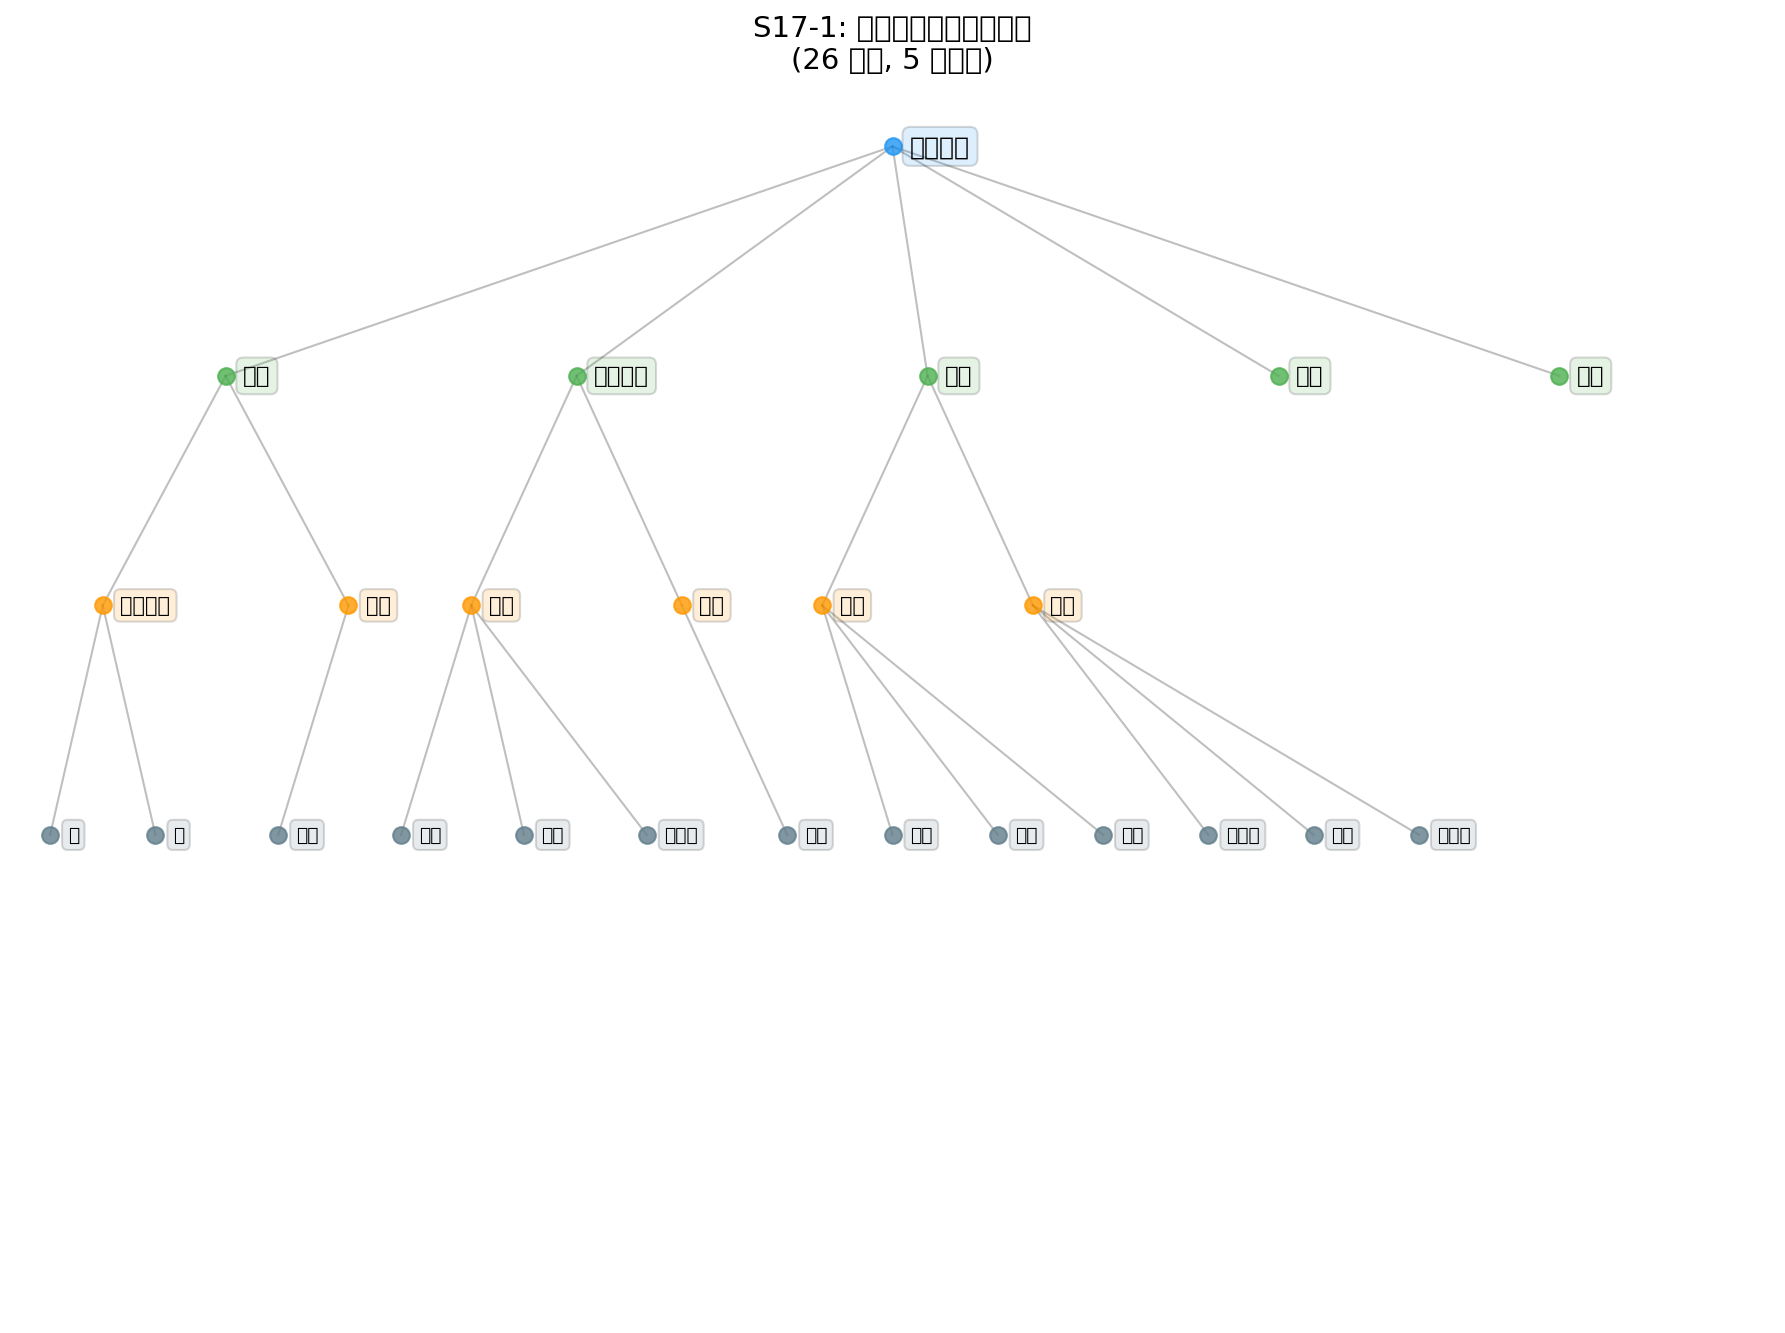
\includegraphics[width=0.6\linewidth,height=\textheight,keepaspectratio]{s17-figures/fig1-concept-hierarchy.png}
\caption{概念层次结构：26个概念在TF-IDF空间中的层次组织}
\end{figure}

\begin{figure}[htbp]
\centering
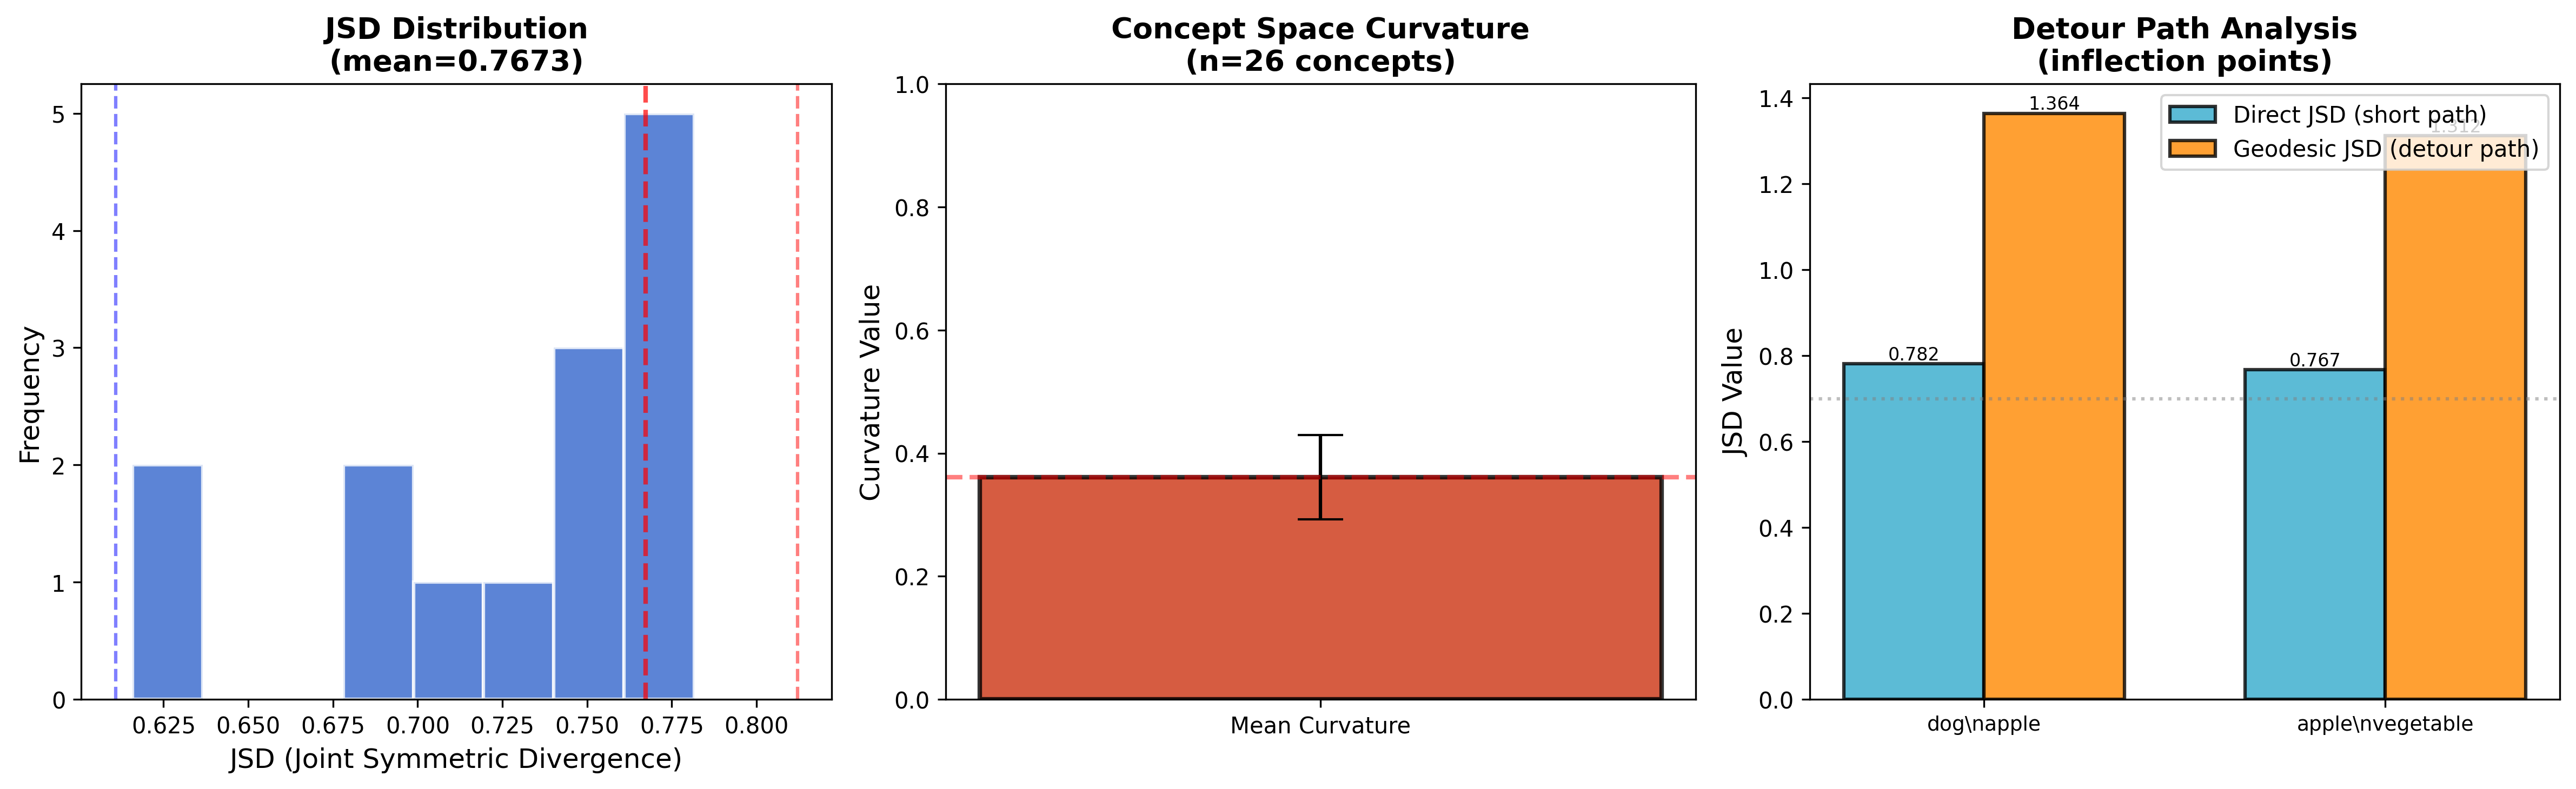
\includegraphics[width=0.8\linewidth,height=\textheight,keepaspectratio]{s17-figures/fig2-statistics.png}
\caption{曲率和JSD统计分布}
\end{figure}

\begin{figure}[htbp]
\centering
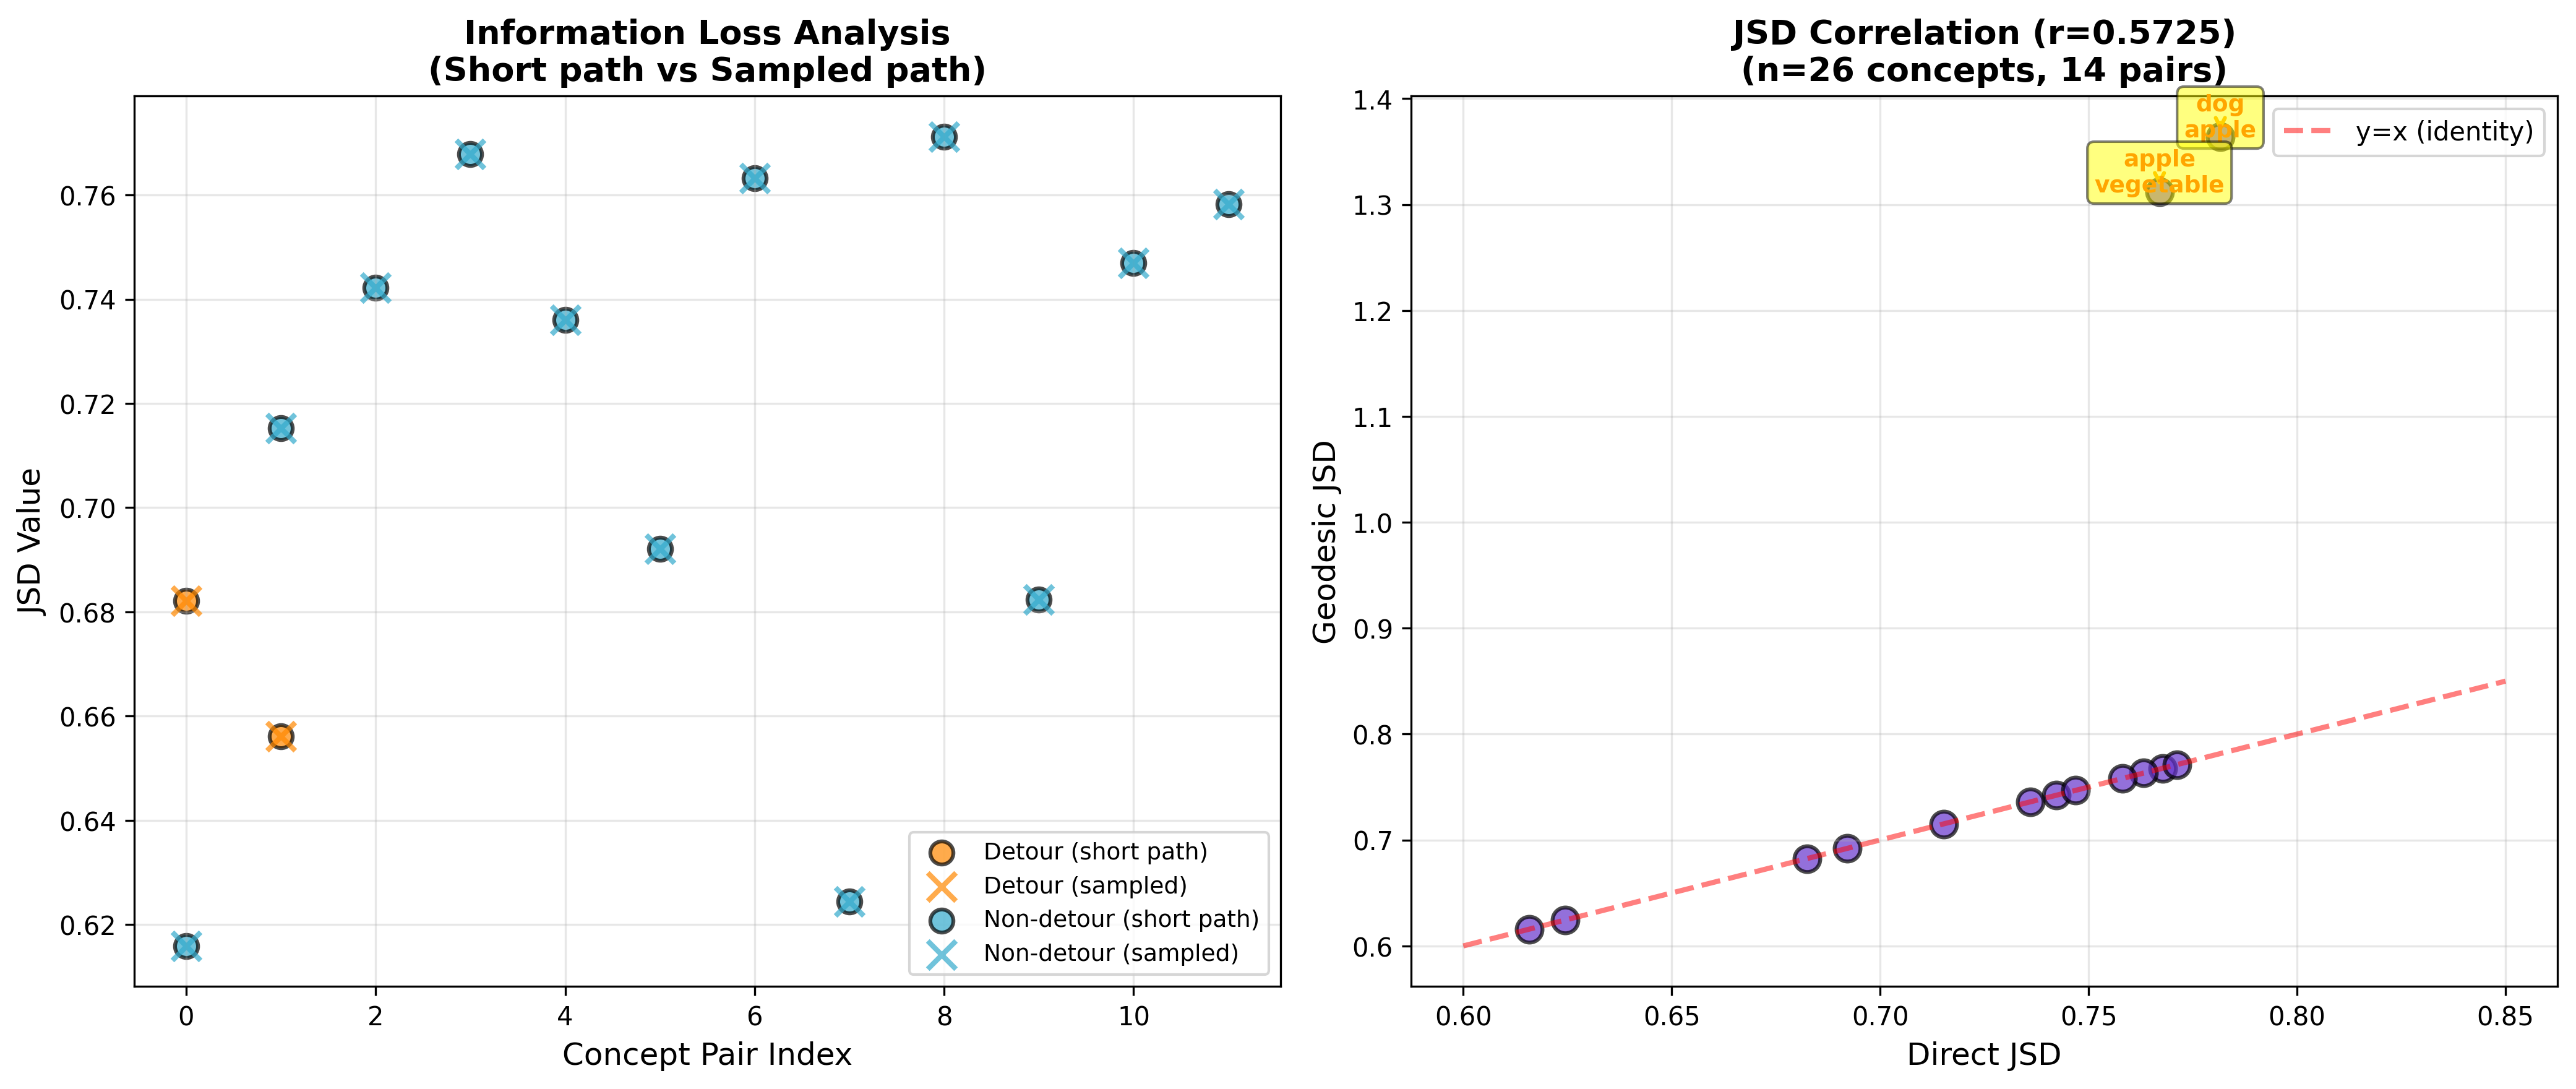
\includegraphics[width=0.8\linewidth,height=\textheight,keepaspectratio]{s17-figures/fig3-detour-analysis.png}
\caption{偏离路径分析：dog\(\to\)apple和apple\(\to\)vegetable的偏离模式}
\end{figure}

\end{document}
